\documentclass[11pt]{article}
\usepackage[utf8]{inputenc} % Para caracteres en espa�ol
\usepackage{amsmath,amsthm,amsfonts,amssymb,amscd}
\usepackage{multirow,booktabs}
\usepackage[table]{xcolor}
\usepackage{fullpage}
\usepackage{lastpage}
\usepackage{enumitem}
\usepackage{multicol}
\usepackage{fancyhdr}
\usepackage{mathrsfs}
\usepackage{wrapfig}
\usepackage[final]{pdfpages}
\usepackage{setspace}
\usepackage{esvect}
\usepackage{calc}
\usepackage{multicol}
\usepackage{cancel}
\usepackage{graphicx}
\graphicspath{ {pictures/} }
\usepackage[retainorgcmds]{IEEEtrantools}
\usepackage[margin=3cm]{geometry}
\usepackage{amsmath}
\newlength{\tabcont}
\setlength{\parindent}{0.0in}
\setlength{\parskip}{0.05in}
\usepackage{empheq}
\usepackage{framed}
%\usepackage{newtxmath}
\usepackage{euscript}
\DeclareMathAlphabet{\mathpzc}{T1}{pzc}{m}{it}
\usepackage[most]{tcolorbox}
\usepackage{xcolor}
\colorlet{shadecolor}{orange!15}
\parindent 0in
\parskip 12pt
\geometry{margin=1in, headsep=0.25in}
\theoremstyle{definition}
\newtheorem{defn}{Definition}
\newtheorem{reg}{Rule}
\newtheorem{exer}{Exercise}
\newtheorem{note}{Note}
\newcommand{\volume}{{\ooalign{\hfil$V$\hfil\cr\kern0.08em--\hfil\cr}}}
\newcommand{\parr}{\mathbin{\|}} % Parralel Symbol
\begin{document}
\setcounter{section}{0}
\setcounter{page}{2}
\setcounter{equation}{0}
\def\thepart{\arabic{part}}
\setcounter{part}{7}
\numberwithin{equation}{part}

 \pagestyle{fancy}
\fancyhf{}
\rhead{Section 7:  Electrothermal Propulsion}
\rfoot{Page \thepage}
\thispagestyle{empty}

\begin{center}
{\LARGE \bf Section 7:  Electrothermal Propulsion}\\
{\large AE435}\\
Spring 2018
\end{center}
\vspace{5mm}
\section{Fundamentals}
\vspace{25mm}
\tableofcontents
\newpage
\subsection{Simple Analysis}
Propellant flexibility leads us to expect high $I_{SP}$. Consider 1D adiabatic nozzle flow from the heating chamber to the nozzle exit. Thus...
\begin{center}
\vspace{50mm}
\textbf{Figure 1:}
\end{center}
\begin{shaded}
\textbf{Stagnation Enthalpy Balance:}

 \begin{equation}
 \begin{aligned}
 h_{oc} = h_{oe}
 \end{aligned}
 \end{equation}
 
  \begin{equation}
 \begin{aligned}
 \frac{1}{2} \, u_e^2+h_e = \frac{1}{2} \, u_c^2 + h_c
 \end{aligned}
 \end{equation}
 
Where
\begin{equation*}
\begin{aligned}
u_e &= \text{The Exit Velocity} \qquad& \text{[m/s]} \\
u_c &= \text{The Chamber Velocity}  \qquad& \text{[m/s]} \\
h_e &= \text{The Exit Enthalpy}  \qquad& \text{[J/kg]} \\
h_c &= \text{The Chamber Enthalpy} \qquad& \text{[J/kg]} 
\end{aligned}
\end{equation*}
 \end{shaded}
If we assume constant specific heats, and negligible inlet speed ($u_c \approx 0$), the exit velocity is:
 
 \begin{shaded}
 \textbf{Exit Velocity}
  \begin{equation*}
 \begin{aligned}
 u_e = \sqrt{2 \, c_p \, (T_c - T_e)}
 \end{aligned}
 \end{equation*}
 Where
  \begin{equation}
 \begin{aligned}
 h_e = c_p \, T_e
 \end{aligned}
 \end{equation}
  \begin{equation}
 \begin{aligned}
  h_c = c_p \, T_c
 \end{aligned}
 \end{equation}
 \end{shaded}
 \newpage
Further, assuming complete expansion ($T_e < < T_c$):
 
   \begin{equation}
 \begin{aligned}
u_e \cong \sqrt{2 \, c_p \, T_c}
 \end{aligned}
 \end{equation}
 
And using
 \begin{framed}
   \begin{equation}
 \begin{aligned}
 c_p = \frac{\gamma \, \Re}{(\gamma - 1) MW}
 \end{aligned}
 \end{equation}
Where
\begin{equation*}
\begin{aligned}
\Re &=8314 \, \frac{J}{Kmol-K}\\
MW &= \text{Molecular Weight} \\
\end{aligned}
\end{equation*} 
 \end{framed}
 
The exit velocity is then:
   \begin{equation}
 \begin{aligned}
u_e \cong \sqrt{\frac{\gamma \, \Re \, 2}{(\gamma -1)\,MW} \, T_c}
 \end{aligned}
 \end{equation}
 \vspace{2mm}
 \begin{framed}
The specific heat $c_p$ is critical: it defines the achievable stagnation enthalpy.  \textbf{For H2,}
\begin{equation*}
\begin{aligned}
T_{oc} &= 3000 \, [K] \, \text{The limit for refractory metals.} \\ \\
C_p &= 2 \times 10^4 \, [J/kg\cdot K] \, \text{at 1atm and 3000K} & \\ \\ 
u_e &= 11 \, [km/s] & \\ \\
I_{SP} &= 1100 \, [sec] &
\end{aligned}
\end{equation*} 
 \end{framed}
 
Assuming an efficiency         $\eta = 60 \%$            	the thrust-to-power ratio of this combination is:
   \begin{equation*}
 \begin{aligned}
 \frac{T}{P} = \frac{2 \, \eta}{g_o \, I_{SP}} = 0.11 \, \Bigg[\frac{N}{kWe}\Bigg]
 \end{aligned}
 \end{equation*}
 
So, Electrothermal Propulsion can readily provide
\begin{itemize}
\vspace{-5mm}
\item 3-4x The $I_{SP}$ of bipropellant system
\item 5x The $I_{SP}$ of monopropellant system
\end{itemize}
Typical commsats have 4-5 kW available for propulsion, so this could provide $\sim$0.5 N of thrust.  
 \newpage
 
 
\subsection{Deviation from Ideal Behavior}
The biggest loss factor in Electrothermal Propulsion is \textbf{Frozen Flow Losses}.  Recall our stagnation enthalpy balance:
   \begin{equation}
 \begin{aligned}
 \frac{1}{2} \, u_e^2 = h_{oc} - h_e
 \end{aligned}
 \end{equation}
 
Frozen flow losses results from non-negligible amounts of unrecoverable internal energy, $h_e$.
 
As an example, consider a hydrazine arcjet.  We start with the exothermic decomposition of hydrazine:
    \begin{equation*}
 \begin{aligned}
 3\,N_2\,H_4 \longrightarrow 4 \,N\,H_3 + N_2
 \end{aligned}
 \end{equation*}
 
There's an associated endothermic dissociation of ammonia:
    \begin{equation*}
 \begin{aligned}
2\,N \, H_3 \longrightarrow N_2+3\,H_2
 \end{aligned}
 \end{equation*}
 
In the discharge chamber, there's enough heat and time to drive both to the end products:
    \begin{equation*}
 \begin{aligned}
3\,N_2 \, H_4 \longrightarrow 3 \, N_2+6\,H_2
 \end{aligned}
 \end{equation*}
 Two Extremes: Equillibrium and Endothermic Reactions.
 
If we exhaust this through a nozzle (so T and p drop with axial distance, x), we can get two extremes.  If the flow stays in equilibrium, the ammonia composition rises with axial distance in the nozzle as nitrogen and hydrogen recombine.
\begin{center}
\vfill
\textbf{Figure 2: }Equilibrium Flow
\end{center}
\newpage
But, if the expansion is quick enough that the endothermic reaction doesn't have time to reverse (i.e., release heat into the flow), we have frozen flow.  In this case, the energy tied up in dissociation is unavailable for acceleration of the gas.
\begin{center}
\vspace{70mm}
\textbf{Figure 3: }No Recombination, No Ammonia, Frozen Flow
\end{center}
Note that dissociation is good in Nuclear Thermal Rockets (NTRs):
\begin{itemize}
\item Lower mean molecular weight of exhaust products
\item Increases maximum $I_{SP}$
\end{itemize}
But this is bad in Electrothermal Propulsion thrusters. 

\textbf{Question: }Why?

\textbf{Answer: } Energy cost

NTRs have lots of cheap power, but making up the lost investment means more solar array area for Electrothermal Propulsion (need more electrical power). And thus more dry mass.
\newpage
\subsection{Efficiency Terms}
Frozen flow is one of several losses that can be described by efficiency terms:
\begin{shaded}
\textbf{Frozen Flow Efficiency:}
    \begin{equation}
 \begin{aligned}
 \eta_f = \frac{h_{oc} - h_e}{h_oc}
 \end{aligned}
 \end{equation}
Where
\begin{equation*}
\begin{aligned}
h_{oc} &= \text{Stagnation Enthalpy in the Chamber}\\
h_e &= \text{Enthalpy at the Exit Plane} \\
\end{aligned}
\end{equation*} 
\end{shaded}
 Physically you can think of this as
 
\begin{equation}
 \begin{aligned}
\eta_f = \frac{\text{Power in Fluid "Available" for Thrust}}{\text{Power in Fluid}}
 \end{aligned}
 \end{equation}
 
Some power is also lost by heat-transfer inefficiencies (remember we assumed adiabatic in (7.1)), this is radiated or conducted heat loss from the system, and can be described by:
 
\begin{shaded}
\textbf{Heating Efficiency}
    \begin{equation}
 \begin{aligned}
 \eta_{th} = \frac{\text{Power into Fluid}}{\text{Electrical Power}}
 \end{aligned}
 \end{equation}
 \end{shaded}
 
Non-ideal nozzle flow is another loss (viscosity, heat transfer in the nozzle, profile losses) costs power too, described by the:
\begin{shaded}
\textbf{Nozzle Efficiency}
    \begin{equation}
 \begin{aligned}
\eta_{n} = \frac{\text{Thrust Power}}{\text{Available Power in Fluid}}
 \end{aligned}
 \end{equation}
 \end{shaded}
 
The overall thruster efficiency is the product of these component efficiencies:
 
\begin{shaded}
\textbf{Overall Thruster Efficiency}
    \begin{equation}
 \begin{aligned}
 \eta = \eta_f \,  \eta_{th}\,  \eta_{n} = \frac{\text{Thrust Power}}{\text{Electrical Power}}
 \end{aligned}
 \end{equation}
 \end{shaded}
 
If we can't keep the overall efficiency high, Electrothermal Propulsion systems lose any competitive advantage over chemical rockets.  This is the major challenge in Electrothermal Propulsion thruster development.


\newpage
\subsection{Enthalpy of High Temperature Gas}
In 1-D energy equation for nozzle flow:
    \begin{equation*}
 \begin{aligned}
  \frac{1}{2} \, u_e^2 = \frac{1}{2} \, u_c^2 + (h_c - h_e)
 \end{aligned}
 \end{equation*}
 
The driving term is the specific enthalpy:
    \begin{equation}
 \begin{aligned}
 h \equiv e + \frac{P}{\rho}
 \end{aligned}
 \end{equation}
 
The partial differential of the enthalpy with respect to temperature at constant pressure is the specific heat:
    \begin{equation}
 \begin{aligned}
 c_p = \bigg(\frac{\partial h}{\partial T}\bigg)_P
 \end{aligned}
 \end{equation}
 
 
The enthalpy of a gas mixture depends on its constituents, and on what internal energy modes they have available.  Consider one kg of a diatomic gas.  The original number of molecules is:
    \begin{equation}
 \begin{aligned}
 N_o = \frac{1}{M_A}
 \end{aligned}
 \end{equation}
where $M_A$ is the molecular mass.  (for example, one kg of nitrogen has
 
    \begin{equation*}
 \begin{aligned}
 (N_o)_{N_2} = \frac{1}{2.325867\times10^{-26} \, [kg]} = 2.150\times10^{25} \,[kg^{-1}]
 \end{aligned}
 \end{equation*}
 
If you heat this to a temperature where dissociation and ionization are important, you get:
\begin{itemize}
\vspace{-3mm}
\item \quad $\alpha_2 \, N_o$ \qquad Neutral molecules
\item \quad $\alpha_1 \, N_o$ \qquad Neutral atoms
\item \quad $\alpha_2^+ \, N_o$\qquad Molecular single ions
\item \quad $\alpha_1^+ \, N_o$\qquad Atomic single ions
\item \quad $\alpha_e \, N_o$ \qquad Free electrons 
 \end{itemize}
 Where  $\alpha$'s are species fractions. Note, we ignore multiple ionization levels.
 \newpage
By conservation of atomic particles, we get:
    \begin{equation}
 \begin{aligned}
 \alpha_2 + \alpha_2 ^+ + \frac{1}{2} \, \alpha_1 + \frac{1}{2} \, \alpha_1^+  = 1
 \end{aligned}
 \end{equation}
While conservation of electric charge gives:

    \begin{equation}
 \begin{aligned}
 \alpha_e = \alpha_1^+ + \alpha_2^+
 \end{aligned}
 \end{equation}
 
We want an equation for the Enthalpy of (7.14), so we will start with the $P/\rho$ term, then do the internal energy , e, term.
 
Now that we've defined the species fractions, we can use this in the perfect gas equation of state:

    \begin{equation}
 \begin{aligned}
 \frac{P}{\rho} = ( \alpha_2 + \alpha_2 ^+ + \alpha_1 + \alpha_1^+ + \alpha_e)\, N_o \, k \, T
 \end{aligned}
 \end{equation}
 
Rewriting conservation of atomic particles (7.17) as

    \begin{equation*}
 \begin{aligned}
 \alpha_2 = 1 - \alpha_2 ^+ - \frac{1}{2} \, \alpha_1 - \frac{1}{2} \, \alpha_1^+
 \end{aligned}
 \end{equation*}
(7.19) then becomes:
   \begin{equation*}
 \begin{aligned}
 \frac{P}{\rho} = ( 1 + \frac{1}{2} \, \alpha_1 + \frac{1}{2} \, \alpha_1^+ + \alpha_e)\, N_o \, k \, T
 \end{aligned}
 \end{equation*} 
 
If we substitute in conservation of charge (7.18), we get:

    \begin{equation}
 \begin{aligned}
 \frac{P}{\rho} = ( 1 + \frac{1}{2} \, \alpha_1 + \alpha_2^+ + \frac{3}{2} \, \alpha_1^+)\, N_o \, k \, T \equiv \alpha_P \, N_o \, k \, T\, 
 \end{aligned}
 \end{equation}
 
which we can write in terms of an \textbf{Indicated Factor:} $\bf{\alpha_P}$ .
 
Now we move on to the internal energy, e, term in (7.14).
\newpage
We can consider the specific internal energy, e, for the individual species:
\begin{enumerate}
\item Neutral molecules
 
    \begin{equation}
 \begin{aligned}
 e_2 = \alpha_2 \, N_o \, \Bigg(\frac{3}{2} \, k \, T + \beta_r \, k \, T + \beta_v \, k \, T + \sum_j \beta_j \, \varepsilon_j\Bigg)
 \end{aligned}
 \end{equation}
Where
   \begin{equation*}
 \begin{aligned}
\frac{3}{2} \, k \, T &= \text{Translational Energy for all Molecules}\\
\beta_r \, k \, T &= \text{Rotational Energy for the Rotationally-Excited Fraction, } \beta_r\\
 \beta_v \, k \, T &= \text{Vibrational Energy for the Vibrationally-Excited Fraction, } \beta_v\\
\beta_j &= \text{Electronic Energy Fraction in the $j^{th}$ Excited State}\\
\varepsilon_j &= \text{The Energy of that Electronic State above Ground State}\\
  \end{aligned}
 \end{equation*} 
\item Neutral atoms
    \begin{equation}
 \begin{aligned}
 e_1 = \alpha_1 \, N_o \, \Bigg(\frac{3}{2} \, k \, T + \sum_k \beta_k \, \varepsilon_k\Bigg)
 \end{aligned}
 \end{equation}
 
\item Molecular ions
    \begin{equation}
 \begin{aligned}
 e_2^+ = \alpha_2^+ \, N_o \, \Bigg(\frac{3}{2} \, k \, T + \beta_r^+ \, k \, T + \beta_v^+ \, k \, T + \sum_l \beta_l \, \varepsilon_l\Bigg)
 \end{aligned}
 \end{equation}
 
\item Atomic ions
    \begin{equation}
 \begin{aligned}
 e_1^+ = \alpha_1^+ \, N_o \, \Bigg(\frac{3}{2} \, k \, T + \sum_m \beta_m \, \varepsilon_m\Bigg)
 \end{aligned}
 \end{equation}
 
\item Free electrons
    \begin{equation}
 \begin{aligned}
 e_e = \alpha_e \, N_o \, \Bigg(\frac{3}{2} \, k \, T \Bigg)
 \end{aligned}
 \end{equation}
 \end{enumerate}
Also need to include the specific dissociation energy (the energy tied up in dissociation):
    \begin{equation}
 \begin{aligned}
 e_d = N_o \, \frac{\alpha_1 + \alpha_1^+}{2} \, \varepsilon_d
 \end{aligned}
 \end{equation}
Where
\begin{equation*}
 \begin{aligned}
\varepsilon_d &= \text{Dissociation energy for a single molecule}\\
  \end{aligned}
 \end{equation*} 
 
The 1/2 term exists because       $\varepsilon_d$  	is split between a pair of atom.

Also need to include the specific ionization energy (the energy tied up in dissociation):
    \begin{equation}
 \begin{aligned}
e_i = N_o \, (\alpha_2^+ \, \epsilon_i + \alpha_1^+ \, \epsilon_i' )
 \end{aligned}
 \end{equation}
Where
\begin{equation*}
 \begin{aligned}
\varepsilon_i &= \text{Molecular Ionization Potential}\\
\varepsilon_i' &= \text{Atomic Ionization Potential}\\
  \end{aligned}
 \end{equation*} 
 
Combine all these terms:(7.20), (7.21), (7.22), (7.23), (7.24), (7.25), (7.26), (7.27),  to get :
\begin{shaded}
\textbf{Total Specific Enthalpy of the Mixture}
    \begin{equation}
 \begin{aligned}
h = e + \frac{P}{\rho} &= \alpha_2 \, N_o \, \Bigg[ (5/2 + \beta_r + \beta_v)\, k \, T + \sum_j \beta_j \, \varepsilon_j\Bigg]\\
&+\alpha_1 \, N_o \, \Bigg[\, \frac{5}{2} \, k \, T + \sum_k \beta_k \, \varepsilon_k + \frac{\varepsilon_d}{2}\, \Bigg]\\
&+\alpha_2^+ \, N_o \, \Bigg[ (5/2 + \beta_r^+ + \beta_v^+)\, k \, T + \sum_l \beta_l \, \varepsilon_l + \varepsilon_i\Bigg]\\
&+\alpha_1^+ \, N_o \, \Bigg[\, \frac{5}{2} \, k \, T + \sum_m \beta_m \, \varepsilon_m + \frac{\varepsilon_d}{2} + \varepsilon_i' \,\Bigg]\\
&+\alpha_e \, N_o \, \Bigg[\,\frac{5}{2} \, k \, T\,\Bigg]
 \end{aligned}
 \end{equation}
 \end{shaded}
 %alpha is fraction of particle that has that state. beta is fraction of particle that is in a particular energy state.

Let's now look at how the internal degrees of freedom is affected by temperature.

\begin{shaded}
\textbf{Internal Degrees of Freedom}
 \begin{equation}
 \begin{aligned}
\EuScript{N} = \frac{2 \, c_v}{N_o \, k}
 \end{aligned}
 \end{equation}
 The available energy modes for storing internal energy.
 \end{shaded}
\newpage
\subsubsection{Effect of Temperature on Internal Degrees of Freedom}
\begin{itemize}
\item Monatomic species:
  \begin{center}
 \vspace{50mm}
 \textbf{Figure 4:}
 \end{center}
Monatomic species have just translation giving it just 3 degrees of freedom (3 dimensions to move around). Monatomic species do not have rotation or vibration and so $\EuScript{N}=3$ up until 1000K, then electronic energy modes become important and so the internal degrees of freedom increases. Monatomic species have fewer degrees of freedom, so their specific heats change less over a range of temperatures up to electronic excitation around $10^4$ K.
 
\item Diatomic gas:
   \begin{center}
 \vspace{50mm}
 \textbf{Figure 5:}
 \end{center}
At low temperatures, the internal degrees of freedom for diatomic molecules is just translational. But, as the particle heats up, they start to gain rotational energy and there for $\EuScript{N}$ increases to 5 (because particles can spin in two directions). Continue to heat and vibration is the next energy mode at around 1000-10000K and $\EuScript{N}$ increases to 7. Increasing temperature again and we start to see electronic energy modes. In a diatomic gas, rotation becomes fully-excited at very low temperature (cryogenic temps, a few K), and vibrational excitation in the high 100s of K. 
 \end{itemize}
 \newpage
The adiabatic index,
  \begin{equation}
 \begin{aligned}
\gamma = \frac{c_p}{c_v} = \frac{N_o \, k +c_v}{c_p} = \frac{\EuScript{N}+2}{\EuScript{N}}
 \end{aligned}
 \end{equation}
is  then:
   \begin{center}
 \vspace{45mm}
 \textbf{Figure 6:}
 \end{center}
Finally, note that since          $h \sim N_o$           and             $N_o \sim \frac{1}{m}$     	the specific enthalpy is higher for lower molecular weight gases.
 
The                    $\alpha$ and $\beta$        	fractions adjust to changes in the flow field at rates that are often slower than translational changes (which are fast):
%Translation respond fastest to changes in flow.
 \begin{enumerate}
\item Rotation $\beta_r$, $\beta_r^+$
\begin{itemize}
\item Adjust very rapidly
\item Fully-excited even at cryo temperatures
\end{itemize}
\item Vibration $\beta_v$, $\beta_v^+$
\begin{itemize}
\item Adjusts at a rate that depends on the mode and molecule
\item Some modes several order of magnitude slower than translation or rotation
\item May be only partially excited at EP temperatures
\item Can get significant vibrational nonequilibrium
\end{itemize}
\item Electronic $\beta_j$, $\beta_k$, $\beta_l$, $\beta_m$
\begin{itemize}
\item Adjusts at rates depending on density and temperature
\item Optical thinness results in loss of radiative equilibrium
\item Higher levels may be sparsely populated and thus negligible
\end{itemize}
%Dissasociation and ionization are slowest of all to respond.
\item Dissociation $\alpha_1$, $\alpha_2$
\begin{itemize}
\item Need collisions with        $\varepsilon \approx \varepsilon_d$         	so slow to adjust
\item Rates highly dependent on density, $\frac{\varepsilon_d}{kT}$
\end{itemize}
\item Ionization $\alpha_1^+$, $\alpha_2^+$
\begin{itemize}
\item Needs        $\varepsilon \geq \varepsilon_i$         	so slow to adjust %energies greater than ionization energy.
\end{itemize}
 \end{enumerate}
 \newpage
 \begin{framed}
 \textbf{Example: }Assume we have $H_2$ at equilibrium with a pressure of 0.01 atm and temperature of 3000K. The gas is at a dissociation of 60$\%$. What is the enthalpy of this hydrogen gas?%We can calculate 

  \begin{equation*}
 \begin{aligned}
\alpha_2  &= (1 - 0.6) = 0.4 &\qquad& \text{Fraction of Neutral Molecules}\\
\alpha_1  &= 2(0.6) = 1.2 &\qquad& \text{Fraction of Atoms}\\
\alpha_p  &= (0.4 + 1.2) = 1.6 &\qquad& \text{Fraction of Particles} \\
 \end{aligned}
 \end{equation*}
 
 At this temperature, there is lots of vibrational excitation, little electronic excitation, so the combustion chamber enthalpy is (7.28):
 
 For atoms, we only have translation, there are no ions present at 3000K. If we were to do SAHA equation, we would see that the ionization fraction would in fact be very small. We would have to double the temperature in order to see ionization.
 
  \begin{equation}
 \begin{aligned}
 h_c = N_o \Bigg[\alpha_2 \Bigg(\frac{9}{2}kT\Bigg)+\alpha_1 \Bigg(\frac{5}{2}kT + \frac{1}{2}\varepsilon_d\Bigg)\Bigg]
 \end{aligned}
 \end{equation}
 
 Assume that all degrees of freedom except dissociation reach equilibrium after complete expansion, so
  \begin{equation}
 \begin{aligned}
 h_e = \frac{1}{2} \, \xi \, \alpha_1 \, N_o \, \varepsilon_d%Defines the exit enthalpy to be this
 \end{aligned}
 \end{equation}
 
where   $\xi$    	is the fraction of the original dissociation remaining at the exit:

 \begin{equation*}
 \begin{aligned}
 \xi &= 0 &\qquad& \text{Equilibrium Flow}\\
 \xi &= 1 &\qquad& \text{Frozen Flow}\\
 \end{aligned}
 \end{equation*} 
 
Solving energy equation for exhaust speed gives:

  \begin{equation*}
 \begin{aligned}
 \frac{1}{2} \, u_e^2 = h_c - h_e
 \end{aligned}
 \end{equation*}
  \begin{equation*}
 \begin{aligned}
 u_e = \left\{\begin{matrix}
1.95 \times 10^4 &,& \xi = 0 &,& \text{Equilibrium Flow}\\ 
1.10 \times 10^4 &,& \xi = 1 &,& \text{Frozen Flow}
\end{matrix}\right.
 \end{aligned}
 \end{equation*}
 
We should expect higher energies with equilibrium flow compared to frozen flow. Hydrogen atoms have recombined and released some of that disassociation energy as translational energy.
  
Dissociation increases $c_p$ (and thus enthalpy) but the increased enthalpy may not be recoverable (frozen flow loss). The gas may expand out so fast that there is no time for the energy to change modes and be released into the exchanged flow.
   \end{framed}
Jahn suggests three ways to avoid frozen-flow losses:
\begin{enumerate}
\item Increase nozzle length (which runs into practical scaling limits, increased weight, and viscous losses). If we make the nozzle longer, then the flow remains in the nozzle longer and then the particles have more time to change energy modes.
\item Operate at higher pressure (to increase the rate of recombination). Jahn's figure 6-3 shows how the complete frozen flow efficiency varies with specific impulse for hydrogen  (the worst-case frozen flow efficiency, with no recombination at all).  Note that higher pressure does help to control frozen-flow losses.\\ \\
 \noindent\makebox[\textwidth]{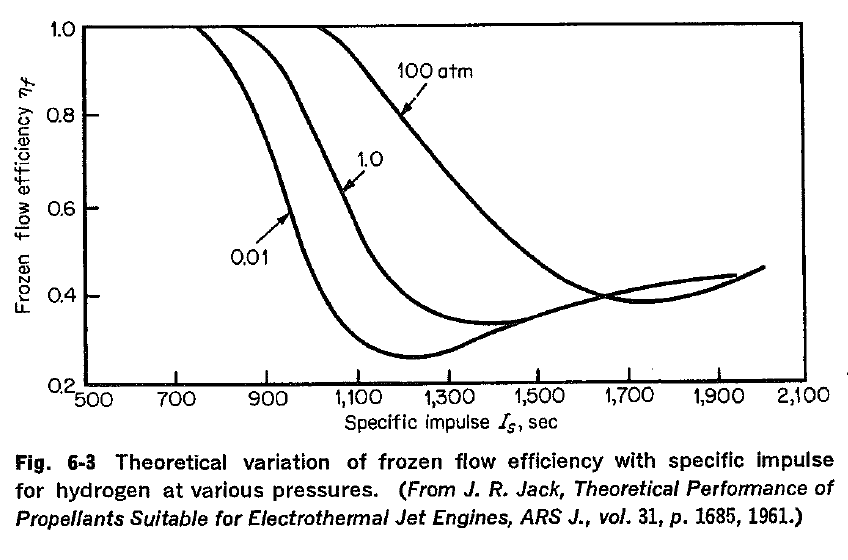
\includegraphics[scale=0.7]{1.png}}
\item Choose a better propellant.   Jahn gives a range of candidates at the end of 6-2. We can choose a propellant that doesn't disassociate as readily, or even a switching to a monopropellant. 
\end{enumerate}
\newpage
\subsection{Equilibrium Composition}
We can define equilibrium composition as the point where forward and backward reactions balance.  For example, the dissociation of hydrogen: 
  \begin{equation*}
 \begin{aligned}
 H_2 \rightleftharpoons 2 \, H
 \end{aligned}
 \end{equation*}
 Showing us that the rate at which $H_2$ is associating is equal to the rate that it is disassociating. Where it is breaking up in the forward reaction and recombining in the backward.
 
The dissociation of hydrogen in an arcjet is at equilibrium when:
  \begin{equation*}
 \begin{aligned}
 \frac{\mathrm{d} }{\mathrm{d} t} (H_2) = \frac{\mathrm{d} }{\mathrm{d} t} (H) = 0
  \end{aligned}
 \end{equation*}
 Where the parenthesis represent the mean concentration [mol/$m^3$]. In this equation, there is no change in the species concentrations while at equilibrium.
 
For the generic reaction
  \begin{equation}
 \begin{aligned}
 A + B \rightleftharpoons C + D %Species A B C D, go back and forth.
 \end{aligned}
 \end{equation}
 
the rate  of change of the concentration of species C is given by:
 
  \begin{equation}
 \begin{aligned}
 \frac{\mathrm{d} }{\mathrm{d} t} (C) = k_{\text{forward}}\,(A)(B) - k_{\text{backward}}\, (C)(D)
 \end{aligned}
 \end{equation}
 
At equilibrium, $\frac{\mathrm{d} }{\mathrm{d} t} = 0 $:
  \begin{equation}
 \begin{aligned}
\frac{(A)(B)}{(C)(D)} = \frac{k_{\text{backward}}}{ k_{\text{forward}}}
 \end{aligned}
 \end{equation}
 
Very generally then, the reaction
  \begin{equation}
 \begin{aligned}
 \nu_A \,A +\nu_B\,B + . . . \rightleftharpoons \nu_C\,C +\nu_D\,D + . . .
 \end{aligned}
 \end{equation}
 Where $\nu_i$ is the number of moles per species. The reaction has an equilibrium constant
 
  \begin{equation}
 \begin{aligned}
 \kappa_P = \frac{P_C^{\nu_C} \, P_D^{\nu_D}}{P_A^{\nu_A} \, P_B^{\nu_B}}
 %Equillbirum constant for a general reation is
 \end{aligned}
 \end{equation}
 
 
where $P_i$ is the partial pressure of species $i$.  For a mixture of perfect gases,
 
  \begin{equation}
 \begin{aligned}
 P_i = \chi_i \, p
 \end{aligned}
 \end{equation}
where
  \begin{equation*}
 \begin{aligned}
\chi_i &= \text{Mole Fraction of Species i }\\
p &= \text{Total Pressure}
  \end{aligned}
 \end{equation*}
 
Thus, the equilibrium constant can be expressed as
 
  \begin{equation}
 \begin{aligned}
 \kappa_P = \frac{\chi_C^{\nu_C} \, \chi_D^{\nu_D} \, ...}{\chi_A^{\nu_A} \, \chi_B^{\nu_B} \, ...} \, P^{(\nu_C+\nu_D+...)-(\nu_A+\nu_B+...)}
 %Has units! Chi is dimensionless but P has units....
 \end{aligned}
 \end{equation}
 
 But this has units! We have units of pressure in this form. 

We can define a \textbf{Dimensionless Equilibrium Constant} for this generic reaction as:

 \begin{equation}
 \begin{aligned}
 \kappa_P = \frac{\chi_C^{\nu_C} \, \chi_D^{\nu_D} \, ...}{\chi_A^{\nu_A} \, \chi_B^{\nu_B} \, ...} \, \Bigg(\frac{P}{P_o}\Bigg)^{(\nu_C+\nu_D+...)-(\nu_A+\nu_B+...)}
 \end{aligned}
 \end{equation}
 
by defining a reference pressure $p_o$ (typically 1 atm).

Note:
\begin{itemize}
\item $\kappa$ is dimensionless
\item $\kappa_p$ is NOT dimensionless
\end{itemize}
For ideal gases, K is a function of Temp only.

Values for $\kappa$ can be found tabulated in numerous combustion texts, e.g., appendix of "Fundamentals of Classical Thermodynamics" by vanWylen and Sonntag. The next page has this table. Note that the values of $\kappa$ in this table are the natural log values. 
\newpage
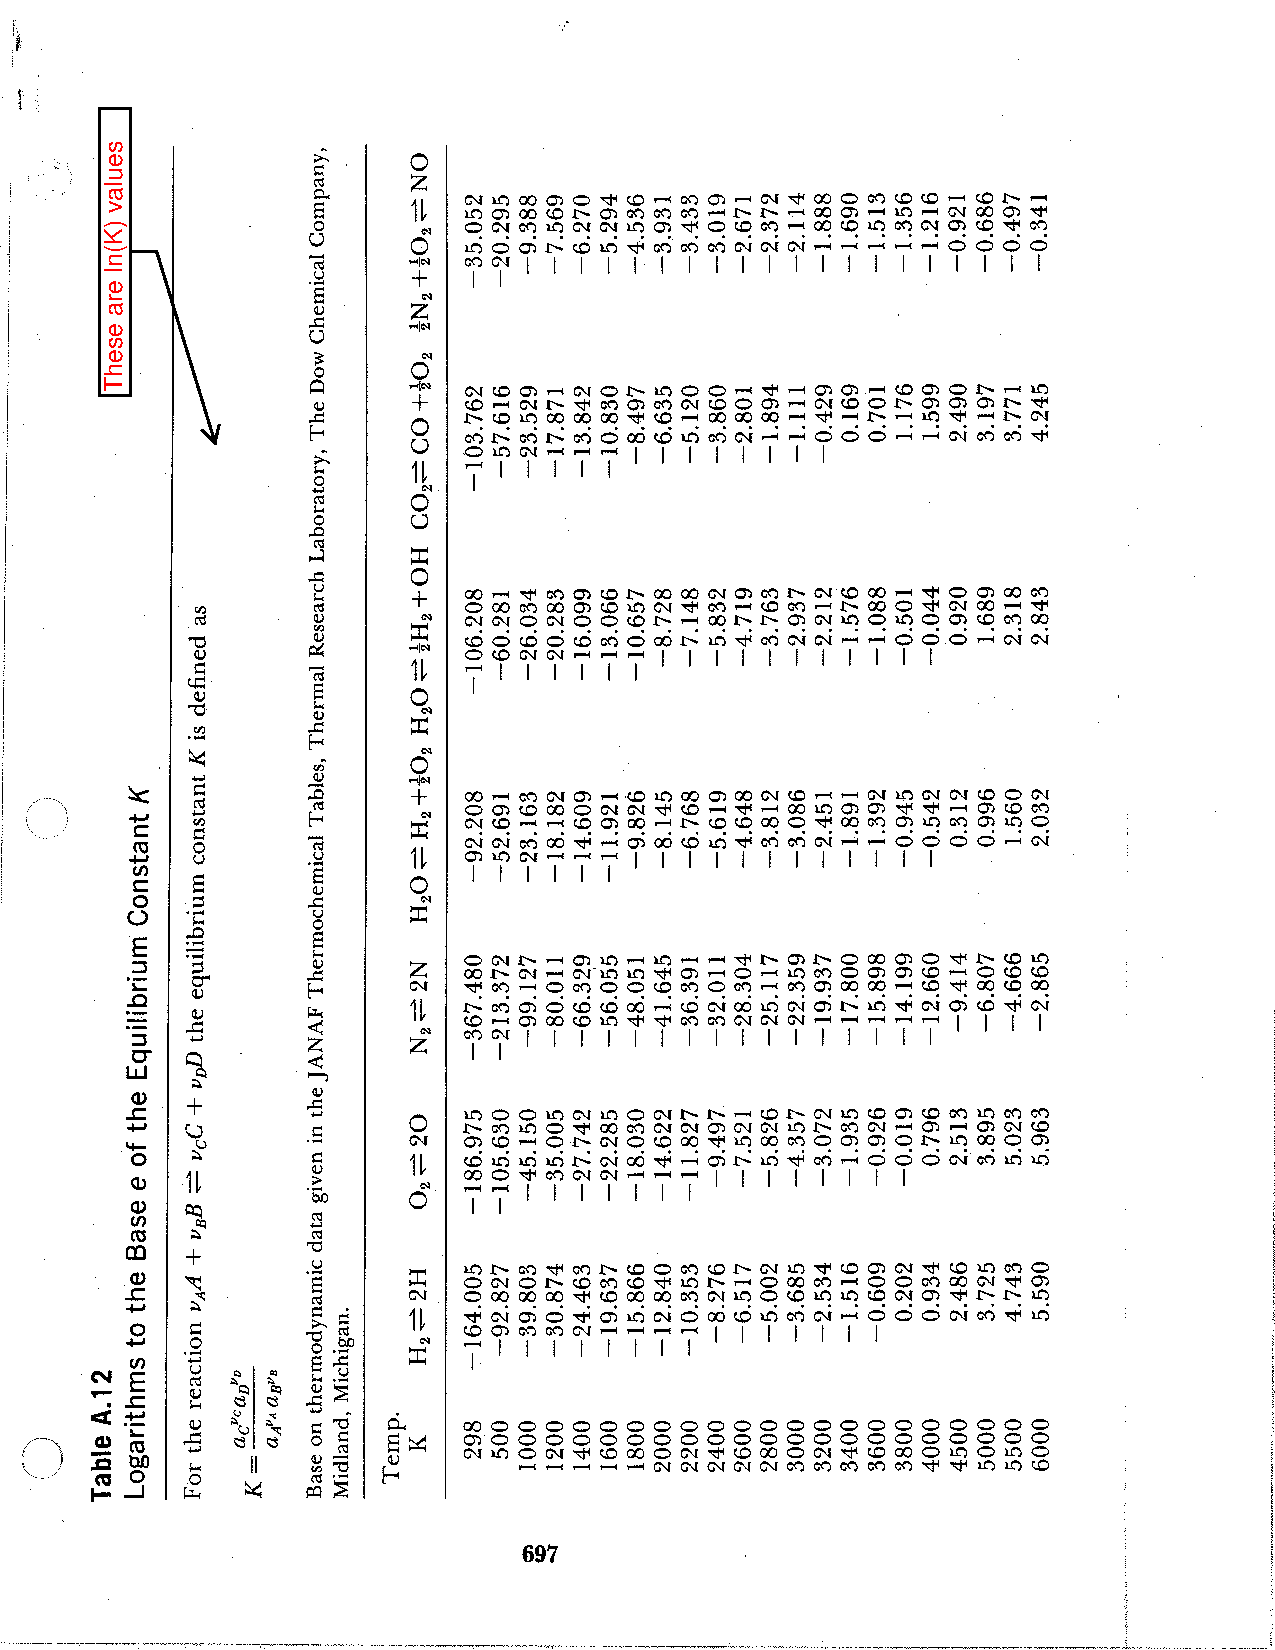
\includepdf{EquilConst.pdf}
 \begin{framed}
\textbf{Example: }Say we have a Hydrogen gas at a temperature of 3000K and pressure of 20 atm. The dissociation reaction
  \begin{equation*}
 \begin{aligned}
H_2 \rightleftharpoons 2 \, H
 \end{aligned}
 \end{equation*}
can be described by the dimensionless equilibrium constant
  \begin{equation*}
 \begin{aligned}
 \kappa = \frac{\chi_H^2}{\chi_{H_2}} \, \Bigg(\frac{P}{P_o}\Bigg)^{2-1} = \frac{\chi_H^2}{\chi_{H_2}} \, 20
 \end{aligned}
 \end{equation*}
 
Now, look up tabulated value of K = K(T) at 3000 K (from the table above):
  \begin{equation*}
 \begin{aligned}
 \kappa \,(3000K) = e^{-3.685} = 2.51\times10^{-2}%FROM TALBLE
 \end{aligned}
 \end{equation*}
so, the mole fraction ratio is:
  \begin{equation*}
 \begin{aligned}
 \frac{\chi_H^2}{\chi_{H_2}} = \frac{2.51\times10^{-2}}{20} = 1.255 \times10^{-3}
 \end{aligned}
 \end{equation*}
 
We still have two unknowns but only one equation. However, from the definition of mole fraction,
  \begin{equation*}
 \begin{aligned}
 \chi_H + \chi_{H_2} = 1
 \end{aligned}
 \end{equation*}
And so
  \begin{equation*}
 \begin{aligned}
 1.255 \times10^{-3} \, (1 - \chi_H) = \chi_H^2
 \end{aligned}
 \end{equation*}
which is a quadratic equation.  The solution has two roots, but only one of them is positive, so:
  \begin{equation*}
 \begin{aligned}
 X_h = 3.482 \times 10^{-2}
 \end{aligned}
 \end{equation*}
and so we have that...

\textbf{At 3000 K and 20 atm pressure, hydrogen is about 3.5$\%$ dissociated}.
  \end{framed}
  \newpage
 \subsubsection{Hydrazine Thruster}
A more relevant example is the hydrazine thruster
 
 \begin{center}
  \vspace{50mm}
 \textbf{Figure 7:}
 \end{center}
These have a long history
\begin{itemize}
\item Early $N_2H_4$ thrusters (Ranger and Mariner midcourse maneuvering engines) used a hypergolic slug to warm a non-spontaneous catalyst bed to temperatures at which $N_2H_4$ decomposed.
\item The Shell 405 catalyst (alumina pellets coated with iridium) was developed in 1962, permitting spontaneous decomposition of hydrazine.
 \end{itemize}
As we saw before, we have two competing reactions.  The first is decomposition of hydrazine:
  \begin{equation*}
 \begin{aligned}
 3 N_2 H_4 \rightleftharpoons 4 N H_3 + N_2 - 336,280 J \qquad \qquad \text{(Exothermic)}
 \end{aligned}
 \end{equation*}
 
If this exothermic reaction was one-way, there would be enough energy to raise the products to an equilibrium temperature of 1650 K.  But at this temperature ammonia dissociates:
   \begin{equation*}
 \begin{aligned}
  2 N H_3 \rightleftharpoons N_2 + 3 H_2 + 184,400 J \qquad \qquad \text{(Endothermic)}
 \end{aligned}
 \end{equation*}
This reaction is endothermic, which drives the equilibrium temperature down.
 
Equilibrium temperature assumes that both reactions have had time to complete!  But the
\begin{itemize}
\item Exothermic reaction is fast, $\sim < 1$ [ms].
\item Endothermic reaction is slow, $\sim 10-100$ [ms].
 \end{itemize}
This means that using hydrazine, we are definitely not going to get equilibrium flow. We are going to get energy loss in disassociation from ammonia.

For a catalyst bed/reaction chamber volume $\volume_{ch}$, we can reduce the residence time to control the dissociation fraction, x.
 \begin{equation*}
 \begin{aligned}
 \tau_{res} = \frac{\rho \, \volume_{ch}}{\dot{m}}
 \end{aligned}
 \end{equation*}
The final reaction then becomes:
    \begin{equation}
 \begin{aligned}
  N_2 H_4 \rightarrow \frac{4}{3}\,(1-x)\,NH_3 + \frac{1}{3}\,(1+2\,x)\,N_2 + 2\,x\,H_2
 \end{aligned}
 \end{equation}
and the enthalpy  balance for an adiabatic reaction is:
    \begin{equation}
 \begin{aligned}
 h_{N_2H_4, \, l \text{ at } 298K} = \frac{4}{3}\,(1-x)\,h_{NH_3}(T) + \frac{1}{3}\,(1+2\,x)\,h_{N_2}(T) + 2\,x\,h_{H_2}(T)
 \end{aligned}
 \end{equation}
which  can be solved for T, given enthalpies.  (subscript $l$ denotes liquid phase).

Need the enthalpies, curve-fits to enthalpy data, using\\

 \[ \scalebox{1.2}{
     \begin{equation}
 \begin{aligned}
h_{NH_3} (\theta) &= \big(-16.83 + 12.35 \theta + 0.983 \theta ^2\big) &\qquad& \Bigg[\frac{\text{kcal}}{mole}\Bigg] & \qquad\\ \\
h_{N_2} (\theta) &= \big(-2.83 + 7.75 \theta + 0.183 \theta ^2\big) &\qquad& \Bigg[\frac{\text{kcal}}{mole}\Bigg]& \qquad\\ \\
h_{H_2} (\theta) &= \big(-1.967 + 6.60 \theta + 0.367 \theta ^2\big) &\qquad& \Bigg[\frac{\text{kcal}}{mole}\Bigg]& \qquad\\ \\
h_{N_2H_4} \big(l, \, 298 \, K\big) &= 12 \, \, \Bigg[\frac{\text{kcal}}{mole}\Bigg] &&&
 \end{aligned}
 \end{equation}
 } \]
  
We can solve for T at various levels of dissociation:\\
 \[ \scalebox{1.2}{
\begin{center}
 \begin{tabular}{c | c} 
Disassociation Level & Equilibrium Temperature \\ 
 x & $T_c$ [K] \\ [0.5ex] 
 \hline
 0.0 & 1659 \\ 
 0.2 & 1502\\ 
 0.4 & 1343\\
 0.6 & 1182\\
 0.8 & 1023\\
 1.0 & 863\\[1ex] 
 \hline
\end{tabular}
\end{center}
 } \]
 
For comparison, the equilibrium composition at $\sim$1000 K is
 \begin{itemize}
 \item $0.23 \% \, NH_3$ at 10 atm
  \item $0.68 \% \, NH_3$ at 20 atm
 \end{itemize}
 
So, if allowed to equilibrate, ammonia would nearly completely dissociate.
 
Dissociation:
\begin{itemize}
\item Decreases chamber temperature $T_c$, but also
\item Decreases the mean product mass (molecular weight) %H atoms are less massive than h2 moleuces
\end{itemize}
To see how these competing effects influence $I_{SP}$,we look at values for  $\varepsilon = 50$, $\frac{P_e}{P_c} = 8 \times 10^{-4}$ and Area Ratio of $\sim$50

 \[ \scalebox{1.2}{
\begin{center}
 \begin{tabular}{c  c  c  c  c} 
x & $T_c$ & Adiabatic Index & $\bar{m}$ & $I_{SP}$\\ 
 & [K] & $\gamma$ & [g/mole] & [s] \\ [0.5ex] 
 \hline
 0.0 & 1659 & 1.330 & 19.2 & 229.4\\ 
 0.2 & 1502 & 1.336 & 17.6 & 226.9\\ 
 0.4 & 1343 & 1.342 & 15.8 & 225.4\\ 
 0.6 & 1182 & 1.348 & 14.0 & 223.6\\ 
 0.8 & 1023 & 1.354 & 12.3 & 220.9\\ 
 1.0 & 863 & 1.362 & 10.67 & 216.7\\ [1ex] 
 \hline
\end{tabular}
\end{center}
 } \]
\\
Clearly, best performance for a purely-chemical hydrazine thruster results at minimal dissociation     $x \rightarrow 0$                   	. Design is typically a compromise between:
\begin{itemize}
\item High performance at high $T_c$
\item Long lifetime at low $T_c$
\end{itemize}
Typical choice is to have a disassociation fraction of x$\sim$0.4, 40$\%$. So we compromise between long life and good performance.
 
We'll explore more when we get into resistojets shortly.

\newpage
\subsection{Nozzle Flow}
Electrothermal thrusters use a converging-diverging nozzle to convert high-enthalpy  chamber gases to high-speed supersonic exhaust:
 
 \begin{center}
 \vspace{80mm}
  \textbf{Figure 8:}
 \end{center}
  Here, we see that temperature is high in the chamber and drops as we move to the exit. The velocity experiences the opposite and accelerates as it moves across the chamber.
  
If we describe two planes, x, and y, that are perpendicular to the mean flow direction, we can use simple 1-D compressible flow equations to arrive at area ratio equation:

\begin{equation}
 \begin{aligned}
 \frac{A_y}{A_x} = \frac{M_x}{M_y} \Bigg( \frac{1 + \frac{\gamma - 1}{2} \, M_y^2}{1 + \frac{\gamma - 1}{2} \, M_x^2} \Bigg)^{\frac{\gamma+1}{2\,(\gamma-1)}}
 \end{aligned}
 \end{equation}
 
where  we use Mach number:
   \begin{equation}
 \begin{aligned}
 M = \frac{u}{\sqrt{\gamma \, R \, T}}
 \end{aligned}
 \end{equation}
 Where
  \begin{equation*}
 \begin{aligned}
 R = \text{Specific Gas Constant} = \frac{\Re}{MW}
 \end{aligned}
 \end{equation*}
 
to nondimensionalize the axial velocity component, u.  Note that the species gas constant:
    \begin{equation}
 \begin{aligned}
 R = k \, N_o
 \end{aligned}
 \end{equation}
 \newpage
The most useful way to use this equation is to calculate properties:
\begin{itemize}
\item $A_e$,$M_e$ at the exit
\item $A_t$,$M_t$ at the throat
\end{itemize}
 
 If the throat is choked,  (ie, flow becomes sonic, $M_t = 1$). 
 
 And so:
    \begin{equation}
 \begin{aligned}
  \frac{A_e}{A_t} = \frac{1}{M_e} \Bigg( \frac{2 + (\gamma - 1) \, M_e^2}{\gamma +1} \Bigg)^{\frac{\gamma+1}{2\,(\gamma-1)}}
 \end{aligned}
 \end{equation}

 \noindent\makebox[\textwidth]{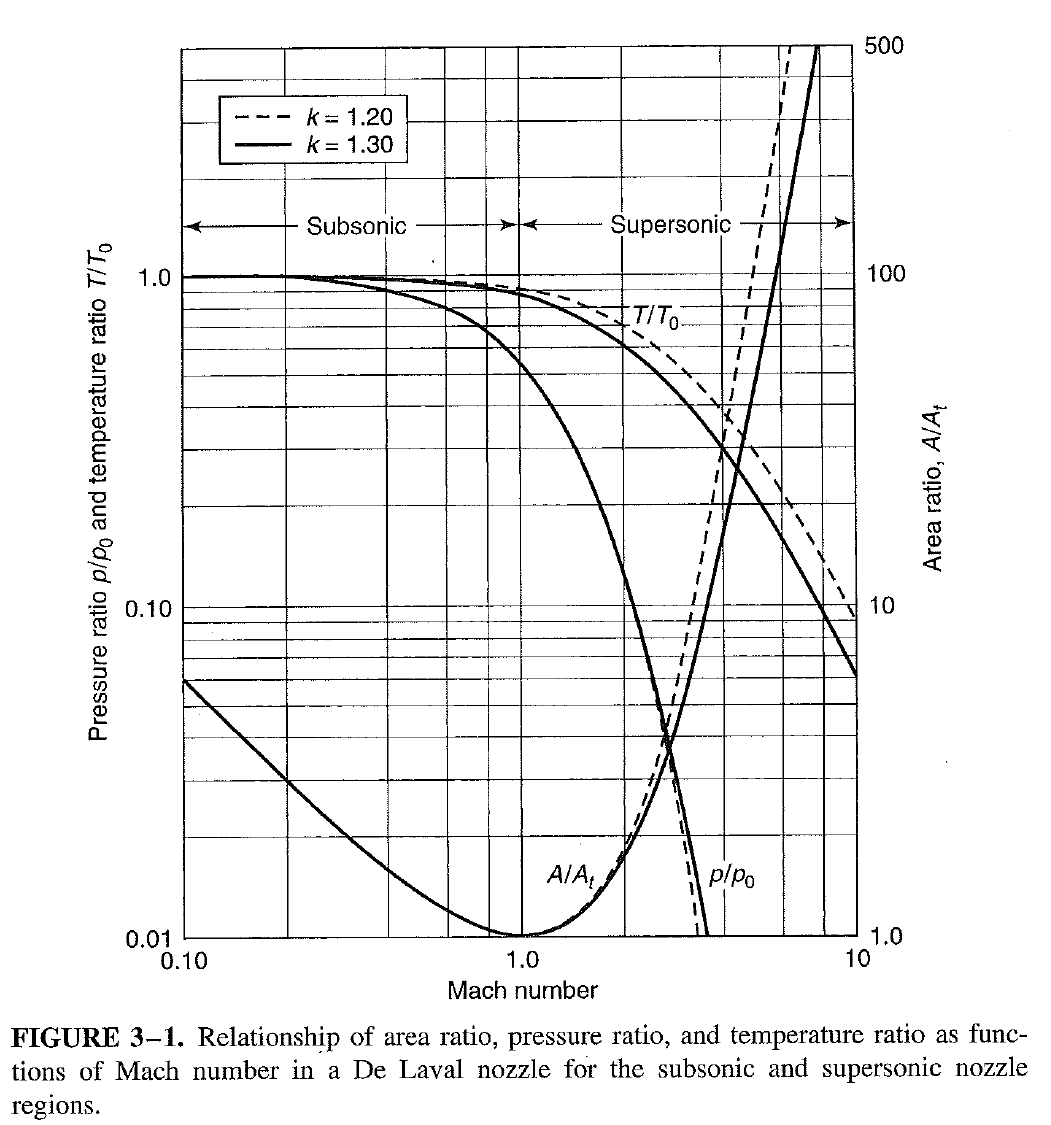
\includegraphics[scale=0.5]{5.png}}%FROM SUTTON TEXT. k = our gamma. 
 \\
 
 Note that as $\gamma$ decreases, we need to increase the area ratio for a fixed exit Mach  number.
 
We can use this equation (7.47) and the isentropic relations to relate exit conditions to fluid conditions in the combustion chamber:

\begin{equation}
 \begin{aligned}
 u_e = \sqrt{\frac{2 \, \gamma \, R \, T_c}{\gamma - 1} \, \Bigg[1 - \Bigg( \frac{P_e}{P_c}\Bigg)^{\frac{\gamma-1}{\gamma}}\, \Bigg] + u_c^2}
 \end{aligned}
 \end{equation}
 
 We can say that the chamber velocity is negligible, $u_c \approx 0$
 
 By inspection, if we want to maximize $u_e$, we need
\begin{itemize}
\item High chamber temperature
\item Low molecular-weight gas
\item Large ratio of chamber pressure to exit pressure
\end{itemize} \\

\noindent\makebox[\textwidth]{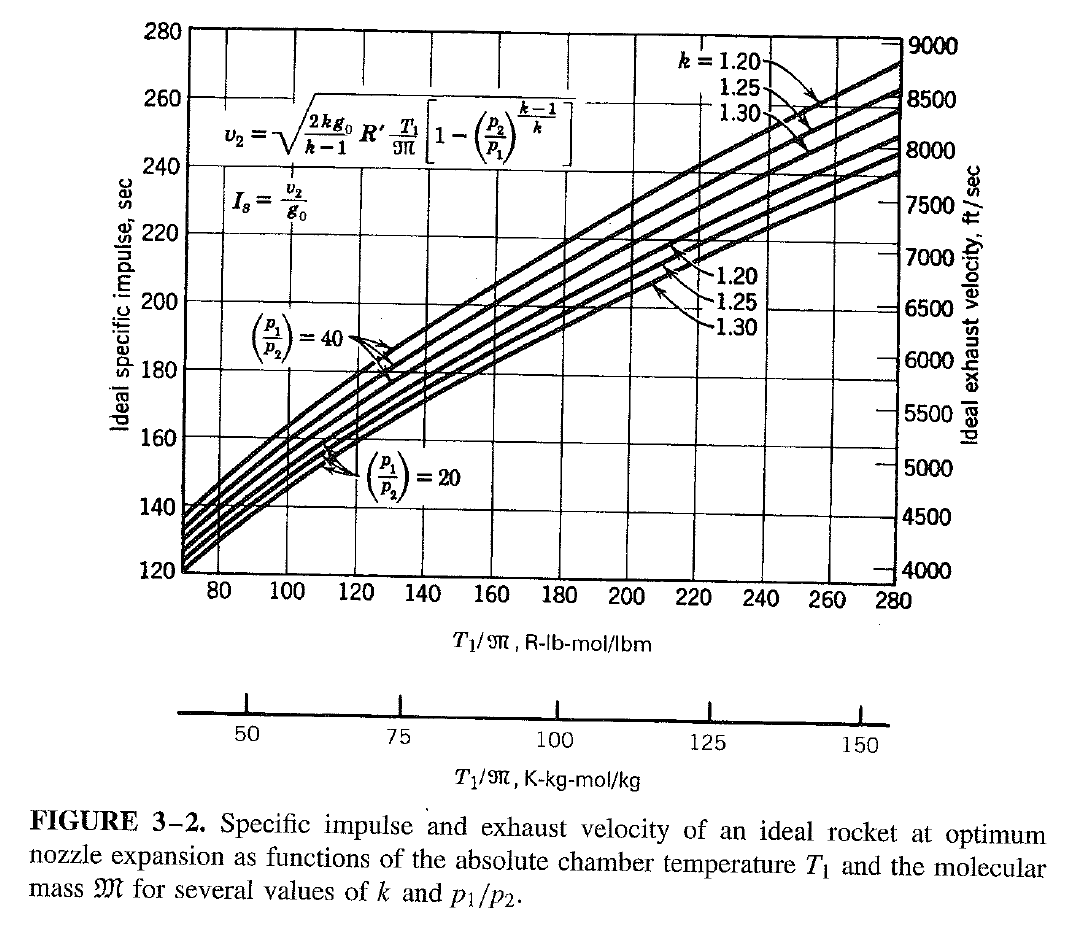
\includegraphics[scale=0.6]{6.png}}%Here is a plot of specific impulse and exauhst velocity as a function of different molecular weights. 
 \\
Note that as $\gamma$ decreases, ideal $I_{SP}$ increases for fixed pressure ratio and chamber temperature.
 
For a perfectly expanded nozzle ($P_e = P_{\infty}$), the thrust is given by:
 \begin{equation}
 \begin{aligned}
 T = \dot{m} \, u_e
 \end{aligned}
 \end{equation}
 
And the specific impulse is given by:
  \begin{equation}
 \begin{aligned}
 I_{SP} = \frac{u_e}{g_o}
 \end{aligned}
 \end{equation}
 
For an imperfectly expanded nozzle, we can define an effective exhaust velocity:
 
  \begin{equation}
 \begin{aligned}
 C_e = u_e + \frac{A_e}{\dot{m}} \,(P_e - P_{\infty})
 \end{aligned}
 \end{equation}
 
And the specific impulse becomes:
  \begin{equation}
 \begin{aligned}
 I_{SP} = \frac{C_e}{g_o}
 \end{aligned}
 \end{equation}
 
For launch vehicles, Isp always increase with altitude.  For ET, $P_{\infty} \sim 0$.
 
\subsubsection*{CHOKED FLOW}
If the pressure ratio across a nozzle is low enough, we will get sonic flow at the throat (min area location).  It's most convenient to calculate the mass flow rate    $\dot{m}$   	based on the throat conditions or to reference the area and velocity to the throat.
 
 \begin{shaded}
 \textbf{Critical Pressure Ratio}
   \begin{equation}
 \begin{aligned}
\frac{P_t}{P_c} = \Bigg(\frac{2}{\gamma +1}\Bigg)^{\frac{\gamma}{\gamma - 1}}
 \end{aligned}
 \end{equation}
Where
  \begin{equation*}
 \begin{aligned}
P_t &= \text{Throat Pressure}
P_c &= \text{Heating Chamber Pressure}
 \end{aligned}
 \end{equation*}
 \end{shaded}
The specific volume       $v = \frac{1}{\rho}$                     at the throat is given by:
 
    \begin{equation}
 \begin{aligned}
\frac{v_t}{v_c} = \Bigg(\frac{\gamma +1}{2}\Bigg)^{\frac{1}{\gamma - 1}} = \frac{\rho_c}{\rho_t}
 \end{aligned}
 \end{equation}
 
while the throat temperature is related to the bulk temperature in the heating zone by:
 
    \begin{equation}
 \begin{aligned}
\frac{T_t}{T_c} = \frac{2}{\gamma + 1}
 \end{aligned}
 \end{equation}
 
Finally, Mt =1, so the velocity in the throat is the speed of sound:
 
    \begin{equation}
 \begin{aligned}
u_t = a_t = \sqrt{\gamma \, R \, T_t}
 \end{aligned}
 \end{equation}
and the mass flow rate:
    \begin{equation}
 \begin{aligned}
\dot{m} = \rho_t \, u_t \, A_t
 \end{aligned}
 \end{equation}
becomes
    \begin{equation}
 \begin{aligned}
\dot{m} = P_c \, A_t \, \sqrt{\frac{\gamma}{R \, T_c} \,  \Bigg(\frac{2}{\gamma +1}\Bigg)^{\frac{\gamma+1}{\gamma - 1}}}
 \end{aligned}
 \end{equation}
 
The area ratio for choked flow at a location, x (subsonic or supersonic), is given by:
 
    \begin{equation}
 \begin{aligned}
\frac{A_t}{A_x} = \Bigg(\frac{\gamma +1}{2}\Bigg)^{\frac{1}{\gamma - 1}} \, \Bigg(\frac{P_x}{P_c}\Bigg)^{\frac{1}{\gamma}} \, \sqrt{\frac{\gamma +1}{\gamma - 1} \, \Bigg[1-\Bigg(\frac{P_x}{P_c}\Bigg)^{\frac{\gamma-1}{\gamma}}\, \Bigg] \, } = \frac{1}{\varepsilon}
 \end{aligned}
 \end{equation}
 
 
where   $\varepsilon$   	is the area ratio, $A_x/A_t$
 
The general velocity ratio is then:
   \begin{equation}
 \begin{aligned}
\frac{u_x}{u_t} = \sqrt{\frac{\gamma +1}{\gamma - 1} \, \Bigg[1-\Bigg(\frac{P_x}{P_c}\Bigg)^{\frac{\gamma-1}{\gamma}} \,\Bigg] \, } 
 \end{aligned}
 \end{equation} 

Therefore, the exit velocity ratio is: 
    \begin{equation}
 \begin{aligned}
\frac{u_e}{u_t} = \sqrt{\frac{\gamma +1}{\gamma - 1} \, \Bigg[1-\Bigg(\frac{P_e}{P_c}\Bigg)^{\frac{\gamma-1}{\gamma}}\,\Bigg] \, } 
 \end{aligned}
 \end{equation}
 
Both relations are shown below (7.59) and (7.60)
\newpage
\begin{center}
  $ $ 
  \end{center}
 \noindent\makebox[\textwidth]{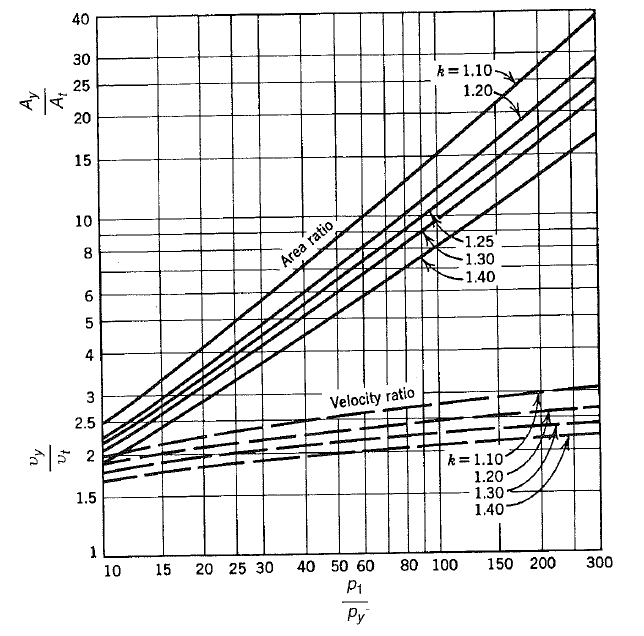
\includegraphics[scale=1]{7.png}}
 \\
 \noindent\makebox[\textwidth]{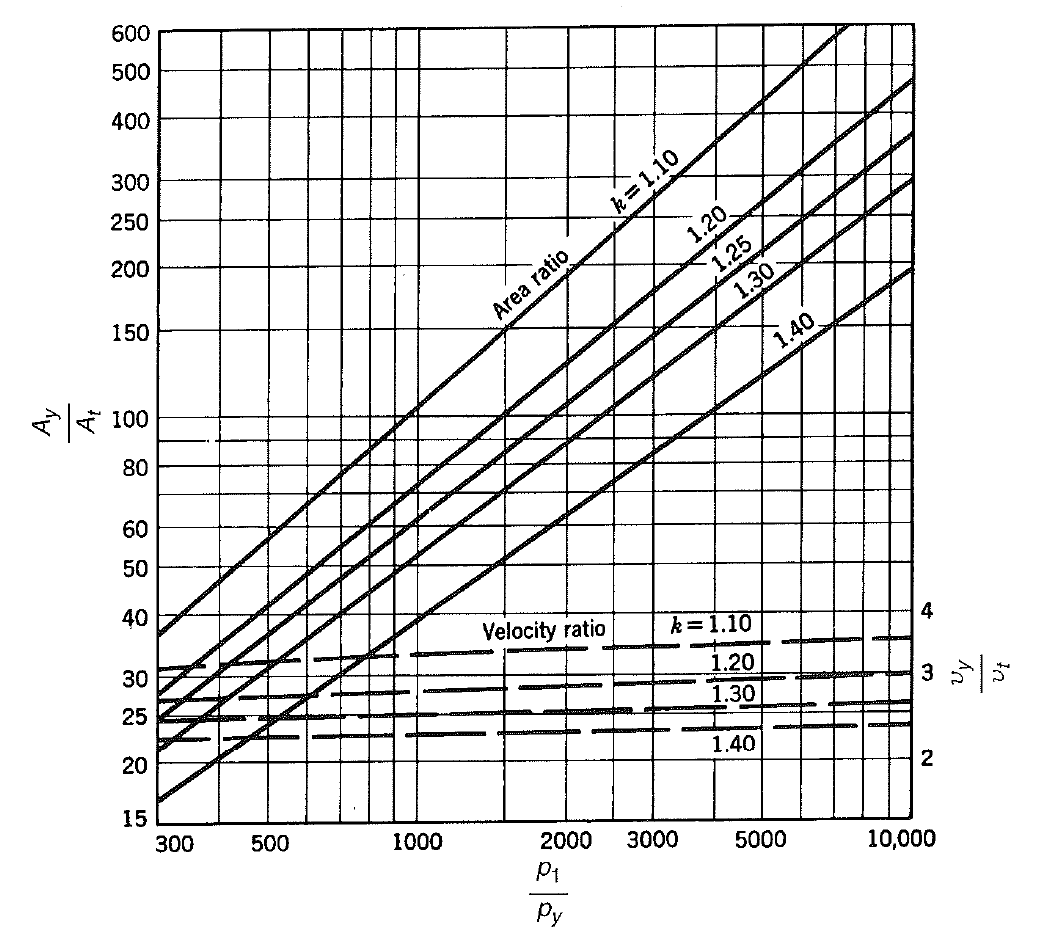
\includegraphics[scale=0.65]{8.png}}
 \\
 
Finally, the thrust
 
    \begin{equation}
 \begin{aligned}
T = \dot{m} \, u_e + A_e \, (P_e - P_{\infty})
 \end{aligned}
 \end{equation}
 
can be written in terms of chamber and exit conditions as:
 
    \begin{equation}
 \begin{aligned}
T =  P_c \, A_t \, \sqrt{\frac{2 \, \gamma^2}{\gamma - 1} \,  \Bigg(\frac{2}{\gamma +1}\Bigg)^{\frac{\gamma+1}{\gamma - 1}} \, \Bigg[1-\Bigg(\frac{P_e}{P_c}\Bigg)^{\frac{\gamma-1}{\gamma}}\,\Bigg] \,} + A_e \, (P_e - P_{\infty})
 \end{aligned}
 \end{equation}
 
This is commonly nondimensionalized as the thrust coefficient:
    \begin{equation}
 \begin{aligned}
C_t = \frac{T}{P_c \, A_t}
 \end{aligned}
 \end{equation}
 
which is shown below for ideal expansion conditions.

\vspace{20mm} 
 \noindent\makebox[\textwidth]{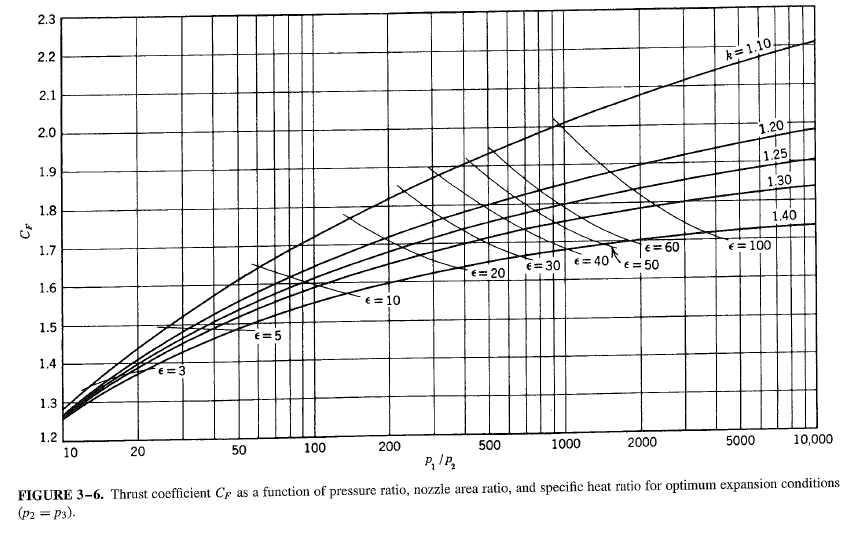
\includegraphics[scale=0.8]{9.png}} \\
 \newpage
 \begin{center}
  $ $ 
  \end{center}
 \vspace{20mm} 
  \noindent\makebox[\textwidth]{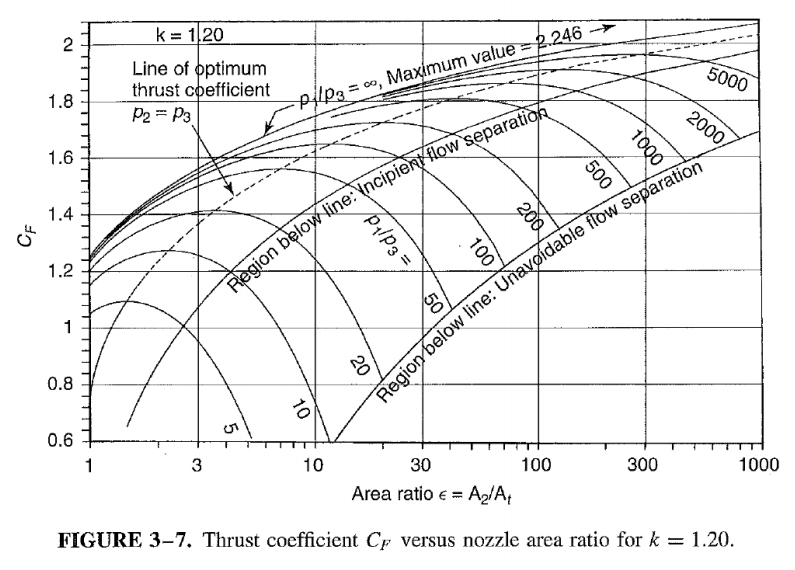
\includegraphics[scale=0.7]{10.png}}\\
   \newpage
\begin{center}
  $ $ 
  \end{center}
 \vspace{20mm} 
   \noindent\makebox[\textwidth]{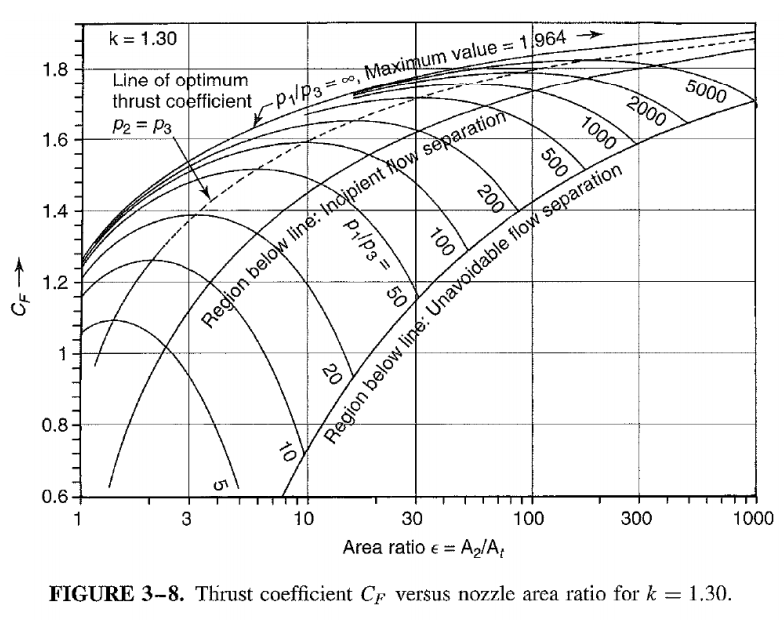
\includegraphics[scale=0.7]{11.png}}\\



\end{document}